\section{Evaluation}
\label{sec:evaluation}

In this section, we evaluate \sys v0.2 on kernel-level and end-to-end performance showing how \sys's design address the challenges of LLM serving. We achieve 29-69\% inter-token-latency reduction compared to Triton backend for LLM serving benchmark, 28-30\% latency reduction for long-context inference, and 13-17\% speedup for LLM serving with parallel generation. We conduct experiments on NVIDIA A100 40GB SXM and H100 80GB SXM GPUs, using CUDA 12.4 and PyTorch 2.4.0 and f16 precision for storage and computation.

\subsection{End-to-end LLM serving performance}

We evaluate \sys with SGLang v0.3.4 \cite{zheng2023sglang} and compare its performance against two settings: SGLang with Triton v3.0 \cite{triton}. The latter is a leading LLM serving engine optimized for NVIDIA GPUs; however, its attention kernels are closed-source, which limits transparency and potential for community-driven improvements. To ensure a comprehensive evaluation, we employ two datasets: the widely-used ShareGPT dataset \footnote{\url{https://huggingface.co/datasets/anon8231489123/ShareGPT_Vicuna_unfiltered/resolve/main/ShareGPT_V3_unfiltered_cleaned_split.json}} and a synthetic workload (Variable) with sequence lengths uniformly distributed between 512 and 2048 tokens. We measure the TTFT(time-to-first-token) and ITL(inter-token-latency) under latency-sensitive online serving settings, the request rate is adjusted to maintain P99 TTFT below 200ms.

\begin{figure}[ht]
    \centering
    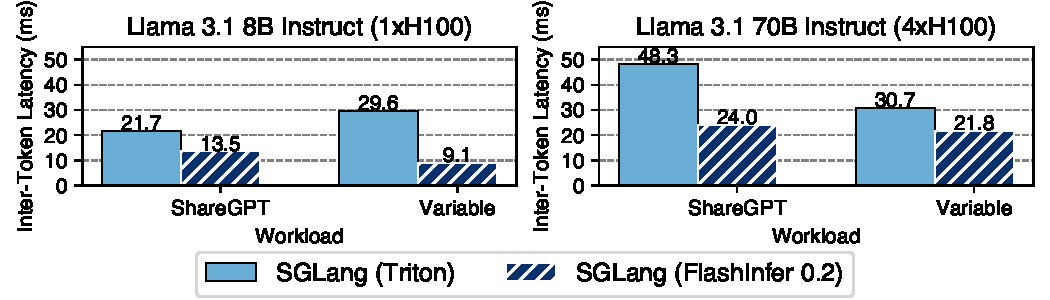
\includegraphics[width=0.45\textwidth]{figures/sglang-itl.pdf}
    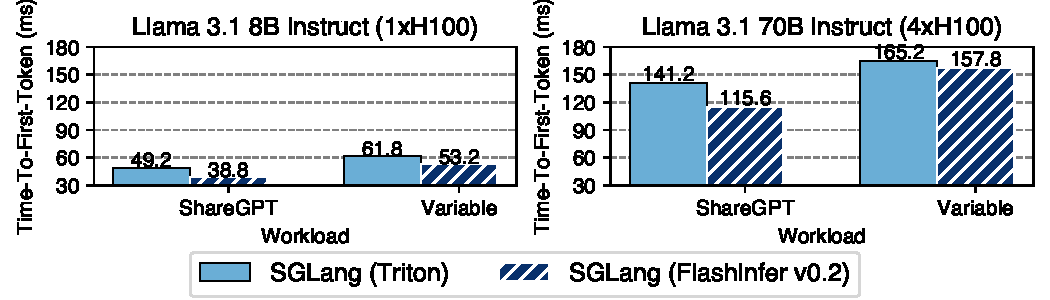
\includegraphics[width=0.45\textwidth]{figures/sglang-ttft.pdf}
    \caption{Medium Inter-Token-Latency (ITL) and medium Time-To-First-Token (TTFT) of SGLang integrated with \sys and Triton.}
    \label{fig:sglang-itl-ttft}
\end{figure}

Figure \ref{fig:sglang-itl-ttft} shows the ITL and TTFT measured on both Llama 3.1 ~\cite{llama31} 8B (on 1xH100) and Llama 3.1 70B (on 4xH100) models. Compared to SGLang with Triton backend, \sys backend shows consistent speedup in all settings.

\subsection{Kernel Performance for Input Dynamism}
\label{eval:input-dynamism}

In this section we measure \sys's generated kernel performance against state-of-the-art open-source FlashAttention library under different sequence length distributions, we use the latest main branch \footnote{Commit: \href{https://github.com/Dao-AILab/flash-attention/commit/c1d146cbd5becd9e33634b1310c2d27a49c7e862}{c1d146c}} which includes both FlashAttention2 and FlashAttention3 kernels. We fix the batch size to 16 and select three different sequence length distributions: constant (1024), uniform (512 to 1024) and skewed (Zipf distribution with average length 1024). For prefill kernels, we enabled causal masking because it's a common setting in LLM serving.

\begin{figure}[ht]
    \centering
    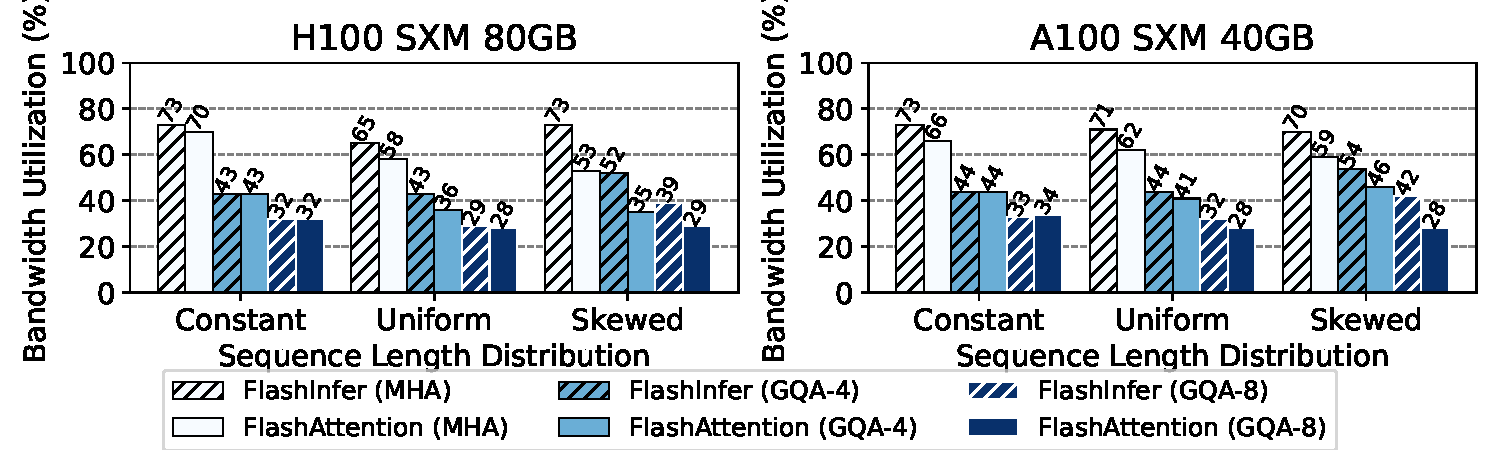
\includegraphics[width=0.45\textwidth]{figures/varlen-decode.pdf}
    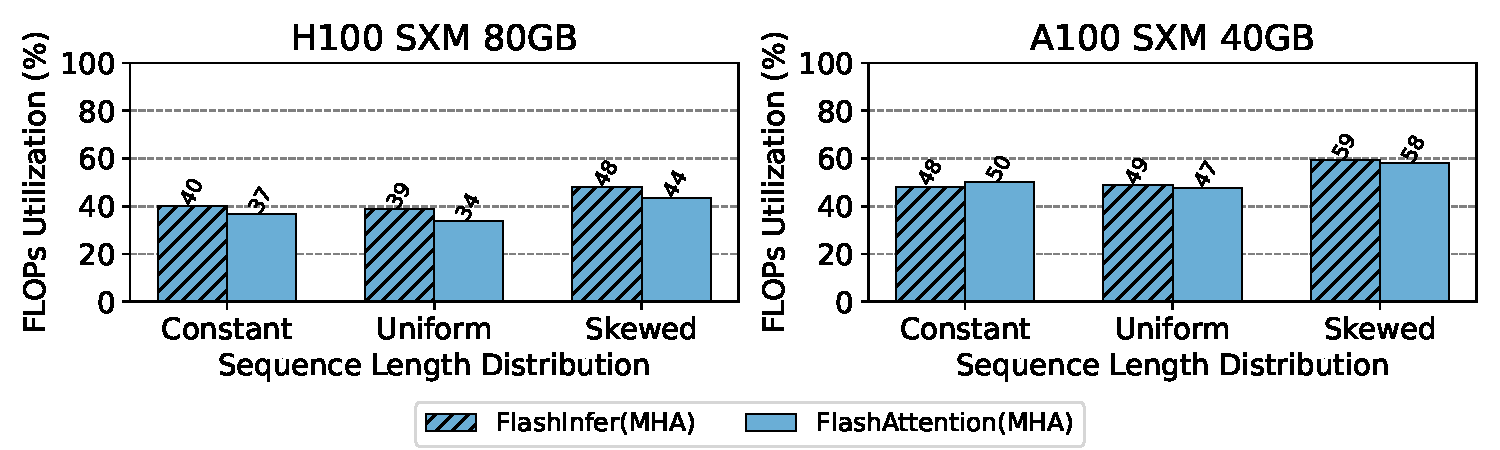
\includegraphics[width=0.45\textwidth]{figures/varlen-prefill.pdf}
    \caption{Achieved bandwidth and FLOPs utilizations (the higher the better) for decode (top) and prefill (down) kernels.}
    \label{fig:varlen}
\end{figure}

Figure \ref{fig:varlen} show the achieved bandwidth and FLOPs utilization for decode and prefill kernels. \sys's kernel significant outperforms FlashAttention kernels in uniform and skewed sequence length distributions because of our  load-balanced dynamic scheduler (section \ref{sec:load-balanced-scheduling}). \sys's decode attention outperforms FlashAttention kernels because our versatile tile size selection (section \ref{sec:tile-size-selection}) and FlashAttention use suboptimal tile size for decoding.

\subsection{Customizability for Long-Context Inference}

In this section, we demonstrate how \sys's customized attention kernels significantly accelerate LLM inference. We focus on Streaming-LLM \cite{xiao2023streamingllm}, a recent algorithm capable of million-token inference with constant GPU memory usage. While Streaming-LLM requires specialized attention kernels for optimal performance, particularly a fused kernel combining RoPE \cite{su2024rope} with attention, \sys can generate such fused kernels with merely 20 additional lines of code for query/key transformations. We compare the performance of \sys-generated fused kernels against un-fused kernels (both \sys's and FlashAttention's) and quantify the end-to-end latency reduction achieved by integrating \sys kernels into StreamingLLM.
\begin{figure}[ht]
    \centering
    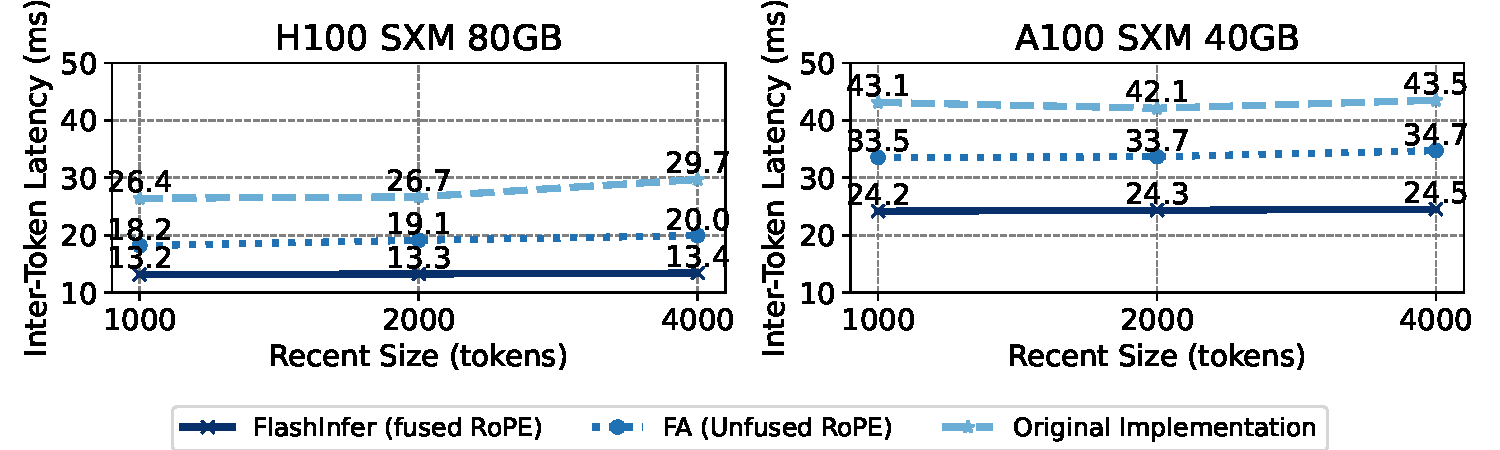
\includegraphics[width=0.4\textwidth]{figures/streaming-llm.pdf}
    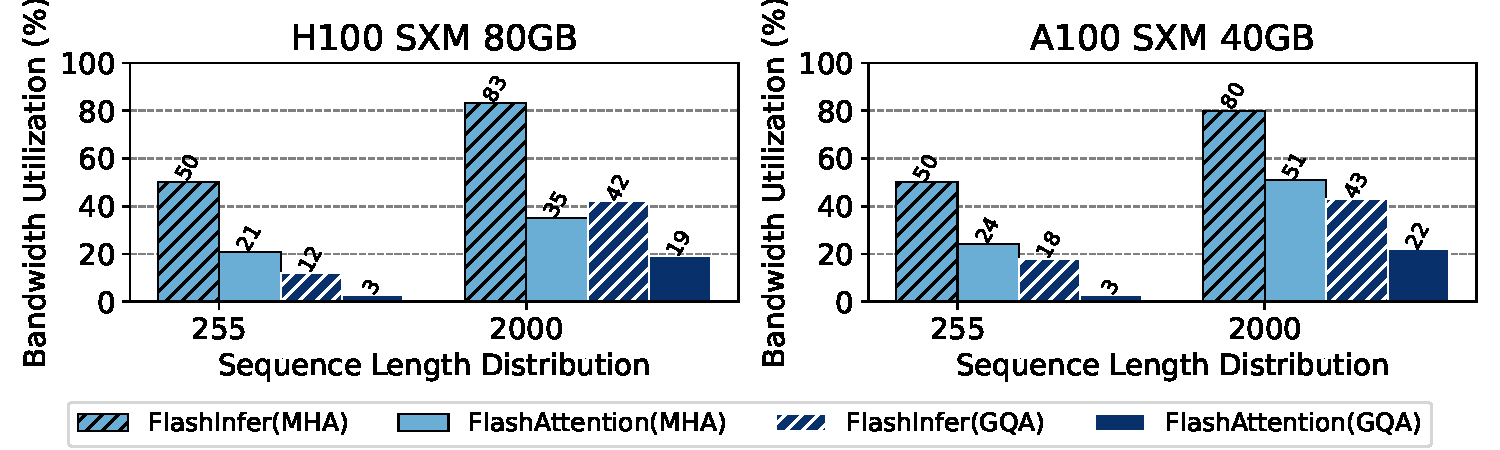
\includegraphics[width=0.4\textwidth]{figures/fused-rope.pdf}
    \caption{Top: End-to-end latency of Streaming-LLM with \sys fused and FlashAttention's unfused kernels, original implementation is included. Down: bandwidth utilization of \sys fused RoPE kernel compared to FlashAttention's unfused kernel.}
    \label{fig:streaming-llm}
\end{figure}

For end-to-end performance, we run Vicuna-13B ~\cite{vicuna2023} inference on MT-Bench ~\cite{zhenbg2023mtbench} dataset and measure the inter-token-latency (ITL) of Streaming-LLM with and without \sys kernels. Figure \ref{fig:streaming-llm} show the ITL of Streaming-LLM with and without \sys fused  kernels on our optimized implementation of Streaming-LLM (we noticed that the original implementation is sub-optimal and have unnecessary overheads). \sys's fused kernel can yield $28-30\%$ latency reduction under different settings (by changing the recent window size of Streaming-LLM). Original implementation is included as a baseline reference. We also show the kernel-level performance comparison between \sys's fused RoPE kernel and the combination of FlashAttention's RoPE kernel and FlashAttention's attention kernel. \sys's fused RoPE kernel achieves 1.6-3.7x higher bandwidth utilization compared to not fusing attention with RoPE, which necessitate the importance of customizability of attention kernels.

\subsection{Parallel-Generation Performance}
\label{eval:memory-heterogeneity}

In this section, we illustrate how the composable formats of \sys can enhance parallel decoding. With parallel generation emerging as a significant task in LLM serving, it offers great utility in LLM agents. The OpenAI API provides an \texttt{"n"} parameter\footnote{\url{https://platform.openai.com/docs/api-reference/chat/create}} to facilitate the generation of multiple tokens simultaneously. As shared prefixes often exist, prefix-caching can significantly boost the efficiency of parallel generation. The composable formats found in \sys (see Section \ref{sec:composable-formats}) allow for the decoupling of attention computation between the shared prefix and the subsequent suffix, which can be leveraged to expedite parallel decoding.
\begin{figure}[ht]
\centering
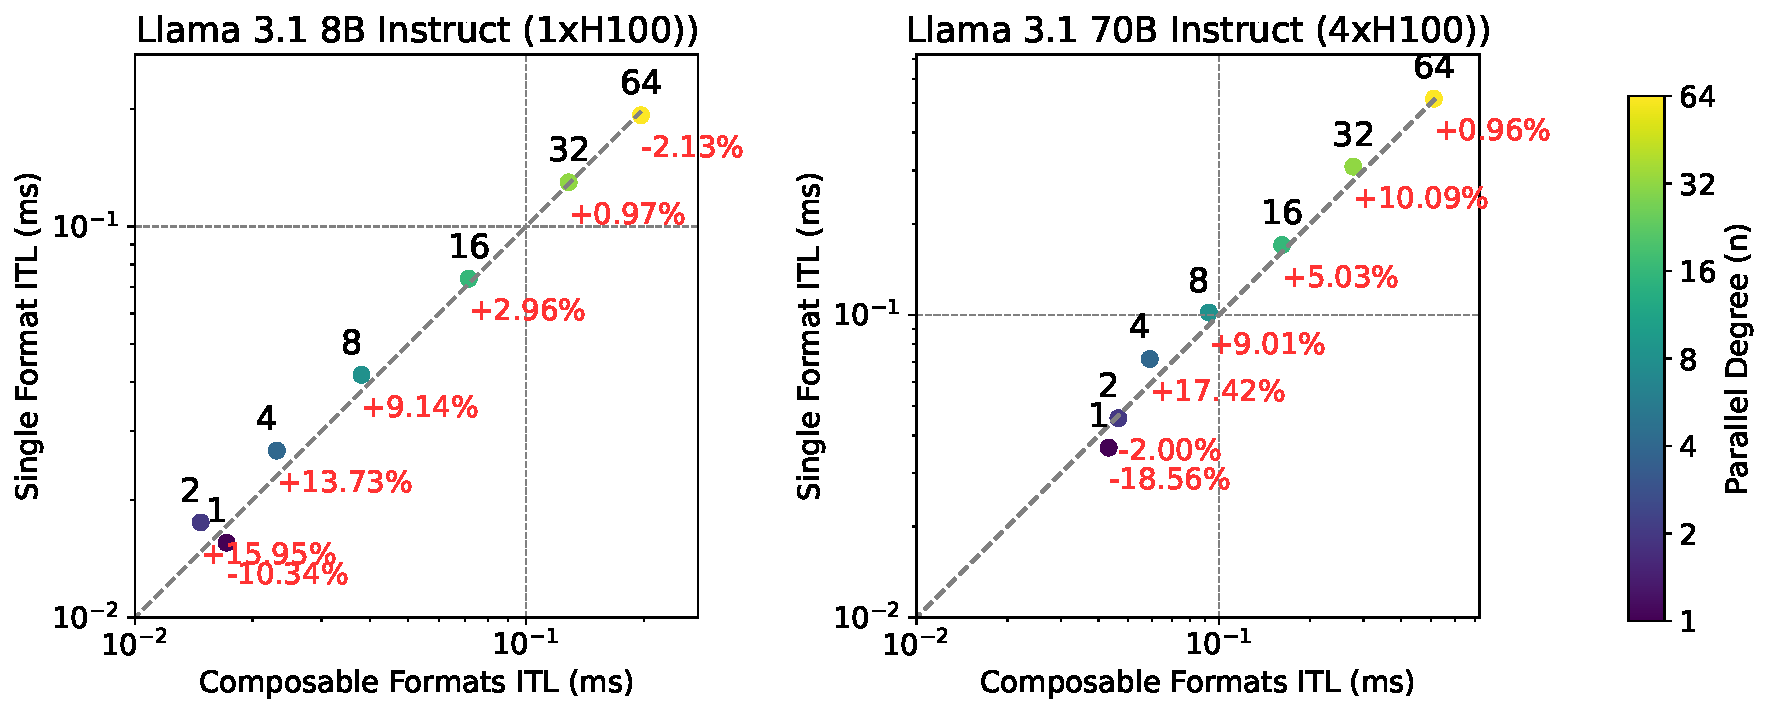
\includegraphics[width=0.4\textwidth]{figures/paragen-itl.pdf}
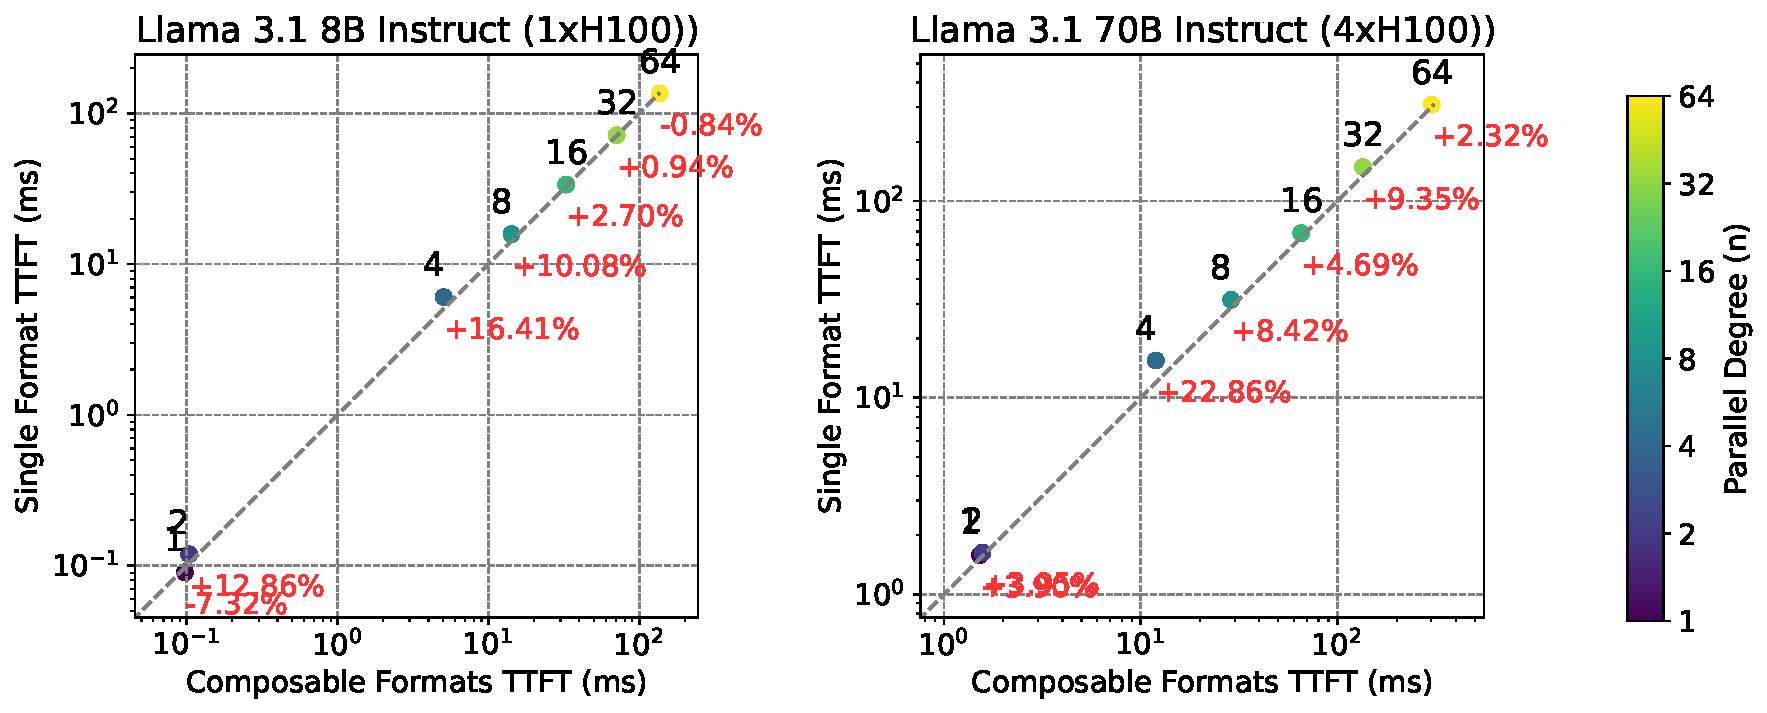
\includegraphics[width=0.4\textwidth]{figures/paragen-ttft.pdf}
\caption{ITL and TTFT of MLC-Engine with and without composable formats during parallel generation, the x-axis refers to composable formats performance, and the y-axis refers to single format performance, if a point is above the diagonal line, it means composable formats outperform single format. Different parallel generation $n$ are shown in different colors.}
\label{fig:parallel-generation}
\end{figure}

We implemented composable formats within MLC-Engine\cite{mlcllm} under a prefix-caching configuration and assessed the performance during parallel generation. Evaluations were conducted on the Llama 3.1 models with 8B and 70B parameters\cite{llama31} using the ShareGPT dataset. With a fixed request rate of 16, we varied the number of parallel tokens over the set ${1, 2, 4, 8, 16, 32, 64}$, comparing these results against MLC-Engine configurations where composable formats were disabled. Figure \ref{fig:parallel-generation} presents the ITL (Inference Time Latency) and TTFT (Time To First Token) results for MLC-Engine both with and without composable formats.

For moderate levels of parallel generation ($4 \leq n \leq 32$), \sys's composable formats yield consistent speedups for both ITL and TTFT. Peak speedups occur at $n=4$, where ITL decreases by $13.73\%$ for the 8B model and $17.42\%$ for the 70B model, while TTFT is reduced by $16.41\%$ for the 8B model and $22.86\%$ for the 70B model. Smaller values of $n$ do not benefit from composable formats due to insufficient increase in block size. For larger $n$, the computation ceases to be dominated by attention processes (especially in the case of ShareGPT with its short sequence length), causing the advantage of composable formats to plateau.
